\documentclass[12pt, a4paper, oneside]{ctexart}
\usepackage{graphicx}
\usepackage{tikz}
\usepackage{amsmath}
\usetikzlibrary{angles,quotes}

\title{Uniswap简明导论}
\author{Splendor White}
\date{\today}

\begin{document}

\maketitle

\section{简介}

Uniswap 是以太坊区块链上的一个去中心化交易所。它既表现出与传统中心化交易所不同的特性,又是去中心化交易所的典型代表。了解其基本运行机制,是认识去中心化金融的基础。

与传统的中心化交易所不同,Uniswap 的交易不需要订单簿,而是由自动做市商根据恒定乘积公式对流动性池进行动态调整,满足交易者的交易需求。流动性提供者可以向流动性池中添加流动性,降低交易者的滑点,并按照份额赚取流动性费用。

Uniswap 具有许多独特的风险,包括但不限于流动性匮乏、无常损失、诈骗、预言机失灵和黑客攻击等。在使用 Uniswap 进行交易与开发的时候需要谨慎处理。

Uniswap 是一个不断发展的交易协议。在 Uniswap V2 中,任意交易对、安全的价格预言机、闪电兑等功能得以实现。在 Uniswap V3 中,集中流动性的引入大大提高了资金利用率。在即将上线的 Uniswap V4 中,挂钩、单例、闪电记账等新元素使得合约可以更加灵活地定制化。

\section{从订单簿到自动做市商}

\subsection{订单簿}

在传统的金融交易过程中,一部分买者和卖者需要在一个公共的\textbf{订单簿}(Order Book)上给出自己的买进报价(Bid)或卖出报价(Ask),这类交易者被称为挂单者(Maker)。其他的买者和卖者可以在订单簿中找到自己心仪的报价,并付给相应的商品或货币,从而完成交易,这类交易者被称为吃单者(Taker)。如图1所示。

\begin{figure}[htbp]
    \centering
    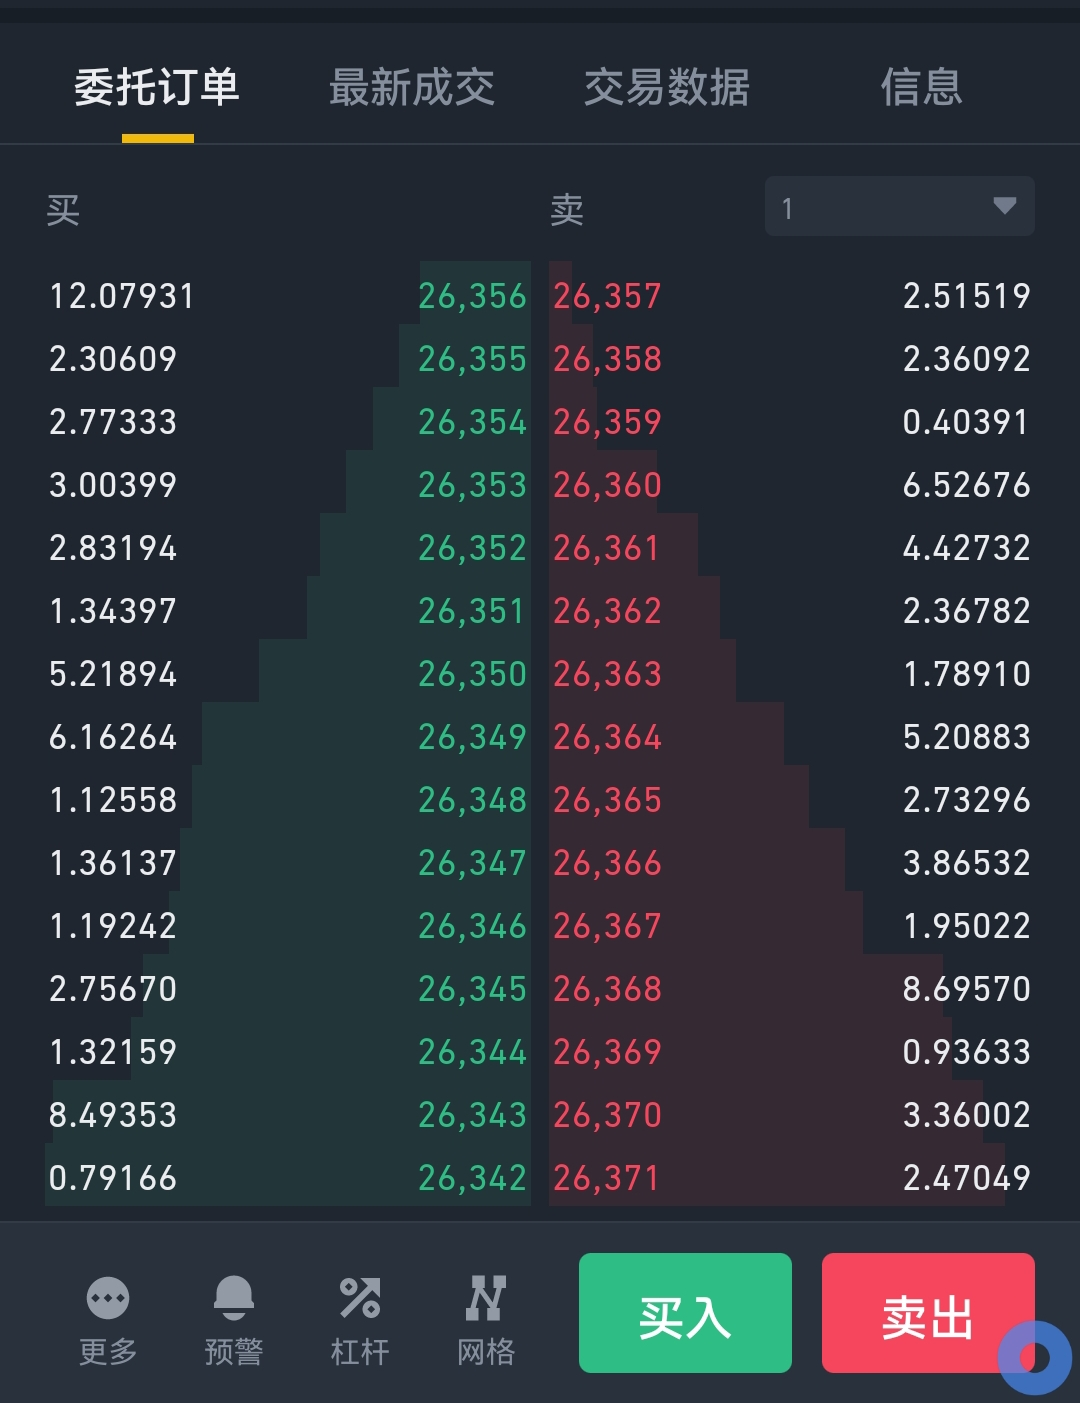
\includegraphics[width=8cm]{订单簿示意图.jpg}
    \caption{订单簿示意图}
\end{figure}

这种交易方式能够确定每一笔订单的成交价格和成交数量,并使得市场深度一目了然。但其流动性是不稳定的,市场深度有时大有时小。而且,由于所有的挂单信息都是公开的,市场操纵者可以根据这些信息使用一定数量的资金来将价格瞬间调整到自己想要的水平。

在订单簿模式下,如果挂单者寥寥无几,成交就会变得异常困难。有没有办法让交易者(无论是买者还是卖者)在任意时刻都能够轻松成交呢?\textbf{自动做市商}(Automatic Market Maker)实现了这一点。

\subsection{自助售货机}

为了理解自动做市商,我们可以先以自助售货机作为一个例子。

考虑一个 24 小时不停工作的可口可乐售货机,里面存放着若干瓶可口可乐和一些零钱。当你想要购买一瓶可乐的时候,你需要将钱放入售货机中,然后售货机就会弹出一瓶可乐。现在,让我们将这个模式推广一下——假设你用某种手段(e.g. 走私或者自制)搞来一些符合质量要求的可口可乐,来到自助售货机面前,希望将可乐卖成零钱。你需要做的就是将可口可乐放入自助售货机中,然后售货机就会将相应的零钱付给你。这样,我们就拥有了一个可口可乐交易所。

假设最开始机器中有 $x_0$ 瓶可乐与 $y_0$ 枚一元硬币,并约定一瓶可乐的价格是 3 元。经过若干次交易之后,机器中有 $x$ 瓶可乐与 $y$ 枚一元硬币。很显然,我们有下面的恒等式:

\begin{equation}
    3x + y = 3x_0 + y_0
\end{equation}

\noindent 这意味着,\textbf{留在机器中的可乐价值与硬币价值的总和是一个定值},我们设 $k=3x_0+y_0$ ,于是有

\begin{equation}
    3x + y = k
\end{equation}

\noindent 将这个式子化为 $y = -3x + k$ ,并画出其函数图像,我们得到一个一次函数(如图2所示)。

\begin{figure}[htbp]
    \centering
    \begin{tikzpicture}
        \draw[-latex] (0,0) -- (2.5,0) node[right] {$x$};
        \draw[-latex] (0,0) -- (0,4) node[above] {$y$};
        \draw[domain=0:1, thick, red] plot (\x, {-\x*3+3});
        \node[left] at (0,3) {$k$};
    \end{tikzpicture}
    \caption{可乐交易所储备图}
\end{figure}

然而,我们可能会遇到这样的窘境:我们一次性想要买的可乐太多了,机器里的可乐根本不够;或者我们一次性想要卖的可乐太多了,机器里的钱根本不够。这其实就是流动性问题。

传统金融中的\textbf{流动性}(Liquidity)是指资产可以迅速、容易地被买卖或兑换成现金的能力。流动性本来是每种资产的特性,例如,我们认为现金的流动性最大,存款、国债、股票、劳动力的流动性次之,而房产、工厂、机器设备的流动性相对而言就小得多,因为我们很难将这些资产变成现金。

在去中心化金融中,流动性的概念发生了一定的改变。笔者认为,Uniswap 中的流动性可以被定义为一个交易对将一定规模的某种资产以很低的成本转换为另一种资产的能力。

解决流动性问题的办法是显然的,我们只需要在机器中额外地投放更多的可乐或硬币即可。投放更多的可乐与硬币,使得机器的总价值从 $k$ 变为 $k'$ ,其中 $k' > k$ 。于是恒等式 (2) 变为

\begin{equation}
    3x + y = k'
\end{equation}

\noindent 相应的函数图像变为

\begin{figure}[htbp]
    \centering
    \begin{tikzpicture}
        \draw[-latex] (0,0) -- (4,0) node[right] {$x$};
        \draw[-latex] (0,0) -- (0,7) node[above] {$y$};
        \draw[domain=0:1, thick, red] plot (\x, {-\x*3+3});
        \node[left] at (0,3) {$k$};
        \draw[domain=0:2, thick, blue] plot (\x, {-\x*3+6});
        \node[left] at (0,6) {$k'$};
        \draw[->] (0.5,1.5) -- (1.3,2);
    \end{tikzpicture}
    \caption{添加流动性后的可乐交易所}
\end{figure}

通过投放可乐或硬币,自助售货机就可以完成更大规模的交易。我们将这种行为称为\textbf{添加流动性}。

这个自助售货机,或者说可口可乐交易所,其实就是用一个\textbf{恒定和自动做市商}(Constant-Sum Automatic Market Maker, CSAMM)完成了交易过程,为买者和卖者提供了方便的交易服务。交易所的流动性越大,买者和卖者就能完成越大规模的交易。

\subsection{Uniswap 的恒定积做市商}

可口可乐交易所的例子非常简明,但是它的弊端十分明显——可乐的价格是不能变化的。在真正的金融市场上,资产价格应当随着供求关系的变化产生波动。

我们假设有人用货币 X 和货币 Y 一起建立了一个\textbf{交易对}(Pair),记作 X/Y ,使得任何人都可以使用一种资产交易另一种资产。在这里,我们称 X 为\textbf{基准货币}(Base Currency),称 Y 为\textbf{计价货币}(Quote Currency)。

Uniswap 为两种资产建立起一个\textbf{流动性池}(Liquidity Pool),其中储备有若干 X 和 Y。设 X 的储备数量为 $x$ ,Y 的储备数量为 $y$ ,这两个量是变量。

Uniswap 使用\textbf{恒定积自动做市商}(Constant-Product Automatic Market Maker, CPAMM)实现可变的价格。设建立流动性池的人向池中加入 $x_0$ 个 X 和 $y_0$ 个 Y ,设其乘积为 $k=x_0y_0$ 。如果不添加或移除流动性,自动做市商控制恒定积公式

\begin{equation}
    xy=k 
\end{equation}

\noindent 恒成立,也就是说 $x$ 与 $y$ 的变化始终成反比例关系,保持其乘积是定值。

$x$ 与 $y$ 相对数量的变化反映了价格(汇率)的变化,而 $xy$ 的变化反映了流动性大小的变化。我们将在下面的一节中详细介绍。

\section{CPAMM的经济原理}

\subsection{价格与储备量的关系}

首先需要声明的是,在笔者看来,价格与汇率并无本质区别。通俗意义上说,价格是一种特殊的汇率,是以法币或稳定币作为计价货币的汇率。生活在传统金融和 Web2 中的人们更倾向于使用美元、人民币、USDT等来作为通用的计价货币,因为这些货币往往有权威背书,购买力相对稳定。这样固然会让讨论问题变得更加方便,但其实也会导致我们束手束脚。

在 Defi 中,我更希望抛弃这样一个垄断了标价权的货币,允许用各种货币作为计价货币。这样,汇率与价格便统一起来。两种货币的汇率,就是以其中一种货币为单位而表示的另一种货币的价格。

在 CPAMM 中,\textbf{基准货币的价格就是两种货币储备量之商的倒数}。体现在储备图上,价格就是储备线上某点与原点连线的斜率。

结合图4,我们可以用数学语言表示,在状态 A 下

$$
p_X = \frac{y_1}{x_1} = \tan \theta
$$

\begin{figure}[htbp]
    \centering
    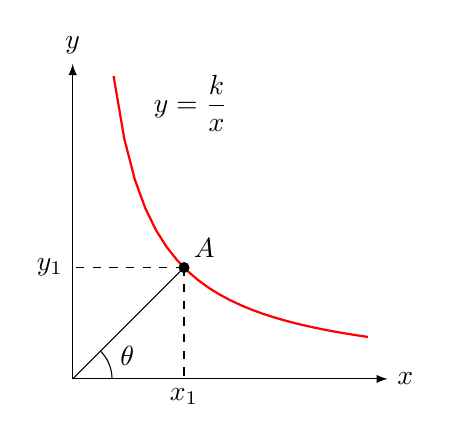
\begin{tikzpicture}
        \draw[-latex] (0,0) -- (4,0) node[right] {$x$};
        \draw[-latex] (0,0) -- (0,4) node[above] {$y$};
        \draw[domain=0.52:3.75, thick, red] plot (\x, {2/\x});

        \fill ({sqrt(2)},{sqrt(2)}) circle (2pt);
        \node[above right] at ({sqrt(2)},{sqrt(2)}) {$A$};

        \coordinate (A) at ({sqrt(2)},{sqrt(2)});
        \coordinate (O) at (0,0);
        \coordinate (B) at ({sqrt(2)},0);
        \coordinate (C) at (0,{sqrt(2)});
        \draw (A) -- (O);
        \pic [draw, pic text=$\theta$, angle eccentricity=1.5] {angle = B--O--A};

        \draw[dashed] (A) -- (B);
        \draw[dashed] (A) -- (C);
        \node[below] at (B) {$x_1$};
        \node[left] at (C) {$y_1$};

        \node at (1.5,3.5) {$\displaystyle y=\frac{k}{x}$};
    \end{tikzpicture}
    \caption{X/Y交易对储备图}
\end{figure}

很显然,如此得到的价格的值域是 $(0,+\infty)$ ,符合实际情况。

读者很可能产生一个疑问:为什么以 Y 为单位 X 的价格能够被表达为 $\displaystyle \frac{y_1}{x_1}$ ?这就是 Defi 的精妙之处。对此,我有两种方式做出解答。

第一种解释是将流动性池看做整个市场的缩影。也就是说,在整个市场上流通着的 X 和 Y 数量之比,就等于流动性池中的 X 与 Y 数量之比。虽然他们数量的绝对大小不同,但比值是相等的。如果人们更加认可 X 的价值,将 X 贮藏起来而不花出去,那么就会使得流通中的 X 数量减少,其价格也就会升高。对于 Y 而言,这条规则同样适用。如果我们认为货币都是平等的,那么数量之商(无论是局部的还是整体的)就是表现人们对货币价值评价的最佳变量。

第二种解释是,CPAMM 能够比较完美地履行以 $\displaystyle \frac{y_1}{x_1}$ 为价格进行交易的职能。我们将在下一节中详细了解这一机制。

有些人认为, CPAMM 的运行完全是依赖于人们的共识、依赖于套利者才能够与其他中心化交易所的价格相锚定。这种观点是片面的。不可否认,套利对于维护去中心化交易所的正常报价至关重要,但这种解释其实是否定了 CPAMM 本身的内在价值,认为 Defi 只不过是完全依附于传统金融的赌场。如果我们继续深入理解 CPAMM ,便会明白,它的价值不是来源于一群信徒的幻想,而是来源于其自身的经济规律。

\subsection{改变价格}

现在激动人心的时刻来了。我们即将见证, CPAMM 究竟是如何在以特定价格完成交易的同时引起价格变化从而反映供求关系的。

我们假设初始状态下流动性池中有 $x_0$ 个货币 X 和 $y_0$ 个货币 Y 。某个交易者准备用 $\Delta x$ 个货币 X 购买一些货币 Y。流动性池收到了这 $\Delta x$ 个货币 X,现在总共有 $x'=x_0+\Delta x$ 个货币 X。为了满足恒定积公式恒成立,新的 Y 储备量 $y'$ 应该满足

\begin{equation}
    x'y'=k
\end{equation}

\noindent 解得

\begin{equation}
    y'=\frac{k}{x'}=\frac{k}{x_0+\Delta x}
\end{equation}

\noindent 显然有 $y' < y_0$ 。实际上,交易所会将一笔数量为

\begin{equation}
    \Delta y = y_0 - y' = y_0 - \frac{k}{x_0+\Delta x}
\end{equation}

\noindent 的货币 Y 发送给交易者。这样,一笔交易就完成了。

首先,让我们从交易者的角度来研究,他的这笔交易是否合他的心意。交易者卖掉了 $\Delta x$ 个货币 X ,买来了 $\Delta y$ 个货币 Y 。如果初状态下价格 $\displaystyle p_X = \frac{y_0}{x_0}$ ,这笔买卖是不是按照价格进行的呢?通过下面的计算我们可以发现,如果交易量相对于流动性池巨大的储备量而言微乎其微,那么这笔交易就是按照价格进行的。

\begin{equation}
\begin{aligned}
    \frac{\Delta x}{\Delta y} 
    & = \frac{\Delta x}{y_0-\frac{k}{x_0+\Delta x}} \\
    & = \frac{\Delta x (x_0+\Delta x)}{y_0 (x_0+\Delta x) - x_0y_0} \\
    & = \frac{x_0 + \Delta x}{y_0} \\
    & \approx \frac{x_0}{y_0} = p_X
\end{aligned}
\end{equation}

如果交易量较大以至于相对于流动性池储备不可忽略,交易者可能会承受多余的成本,这就是去中心化交易所中的\textbf{滑点}(Slippage)。关于滑点的细节,我们将在下一节详细介绍。

接下来让我们从交易所的角度来研究,这笔交易如何改变价格以反映供求关系的变化。交易完成后新的价格 $p_X'$ 满足

\begin{equation}
\begin{aligned}
    p_X' 
    & = \frac{y'}{x'} = \frac{x_0y_0}{(x_0+\Delta x)^2} \\
    & < \frac{x_0y_0}{x_0^2} = \frac{y_0}{x_0} = p_X
\end{aligned}
\end{equation}

\noindent 这意味着新的价格比旧的价格更低。实际上这不难理解。交易者卖出 X 而买入 Y ,实际上是增加了对 Y 的需求与对 X 的供给。货币 X 供过于求导致价格下降,在代数上就体现为 $p_X' < p_X$。

\begin{figure}[htbp]
    \centering
    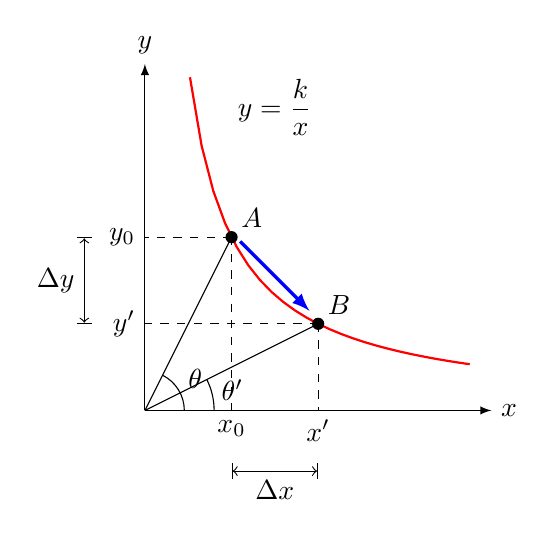
\begin{tikzpicture}[scale = 1.1]
        \draw[-latex] (0,0) -- (4,0) node[right] {$x$};
        \draw[-latex] (0,0) -- (0,4) node[above] {$y$};
        \draw[domain=0.52:3.75, thick, red] plot (\x, {2/\x});
        \node at (1.5,3.5) {$\displaystyle y=\frac{k}{x}$};

        \coordinate (A) at (1,2);
        \coordinate (O) at (0,0);
        \coordinate (B) at (1,0);
        \coordinate (C) at (0,2);
        \fill (A) circle (2pt);
        \node[above right] at (A) {$A$};

        \draw (A) -- (O);
        \pic [draw, pic text=$\theta$, angle eccentricity=1.5] {angle = B--O--A};

        \draw[dashed] (A) -- (B);
        \draw[dashed] (A) -- (C);
        \node[below] at (B) {$x_0$};
        \node[left] at (C) {$y_0$};

        
        \coordinate (D) at (2,1);
        \coordinate (E) at (2,0);
        \coordinate (F) at (0,1);
        \fill (D) circle (2pt);
        \node[above right] at (D) {$B$};

        \draw (D) -- (O);
        \pic [draw, pic text=$\theta'$, angle eccentricity=1.3, angle radius=25] {angle = E--O--D};
        
        \draw[dashed] (D) -- (E);
        \draw[dashed] (D) -- (F);
        \node[below] at (E) {$x'$};
        \node[left] at (F) {$y'$};

        \draw[-latex, very thick, blue] (1.1,1.95) -- (1.9,1.15);
        \draw[|<->|] (1,-0.7) -- node[below] {$\Delta x$} (2,-0.7);
        \draw[|<->|] (-0.7,1) -- node[left] {$\Delta y$} (-0.7,2);

    \end{tikzpicture}
    \caption{交易改变了价格}
\end{figure}

图 5 是对这笔交易的夸张化演绎。通过几何方法,我们也可以由 $\tan \theta' < \tan \theta$ 得出价格下降了。

一次交易可能并不会对价格产生显著的影响,但是诸多交易者的合力将会共同组成一只看不见的手,推动价格朝着特定方向持续演化,直到形成新的均衡。

交易使得流动性池的状态从 A 点移动到 B 点,改变了交易对的价格,但没有改变储备曲线本身。

\subsection{改变流动性}

通过前面的例子,我们发现,除了 $x$ 和 $y$ ,流动性 $k$ 的大小也是值得研究的对象。

流动性过小有诸多危害:较高的滑点导致交易者付出更高成本,巨鲸可以很轻松地掏空流动性池引起价格剧烈变化,价格对交易过于敏感导致难以精确反映供求信息,交易者减少交易量导致流动性提供者收益下降……

为了鼓励\textbf{流动性提供者}(Liquidity Provider, LP)向流动性池中注入更多资金, Uniswap 协议为每一个交易对设定了一个交易费(通常是 $0.3\%$),作为给 LP 的报酬。交易者向流动性池放入的资金先扣除这一笔交易费,剩余的资金再根据恒定积公式进行交易。交易费将转化为新的流动性,持续累积在流动性池中,直到 LP 决定移除流动性为止。这其实就是一种全自动的再投资。

流动性相关的知识可谓是博大精深,我们这里只讨论两个非常简单的问题:添加或移除流动性会发生什么,以及 LP 的收益是如何分配的。

当第一位 LP 向流动性池存入第一笔资金时,此交易对的价格就由这笔资金中两个货币的数量决定。显然,第一位 LP 不能随心所欲地按照任意比例存入资金。如果其中任意一种货币在市场上已经存在了一个价格,那么 LP 必须尊重这个价格并严格按照这个价格确定存入资金的比例,否则就存在套利空间。如果两种货币都没有已经确定的价格,第一位 LP 存入资金的比例就决定了开盘价。

我们假设第一位流动性提供者存入了 $x_0$ 个货币 X 和 $y_0$ 个货币 Y ,而且这个价格并不存在套利空间,并设 $k_0 = x_0y_0$ 。交易者付出交易费引起再投资, $k$ 会缓慢地增大,但我们先忽略这一点,假设不存在交易费。

若干次交易之后,流动性池中有 $x_1$ 个货币 X 和 $y_1$ 个货币 Y ,且依然满足 $x_1y_1=k$ 。这时,第二位 LP 决定向流动性池中加入 $x_2$ 个货币 X 和 $y_2$ 个货币 Y 。显然,他必须保证 $\displaystyle\frac{x_1}{y_1} = \frac{x_2}{y_2}$ ,否则就会存在套利空间。

我们设 $x'=x_1+x_2, y'=y_1+y_2$ ,新的恒定积可由 $k' = x'y'$ 计算得出,新的恒定积公式为

\begin{equation}
    xy = k'
\end{equation}

显然 $k'>k$ 。

公式 (10) 和公式 (4) 是同一形式、不同规模的反比例函数。在图像上,我们可以发现,新的储备曲线是由旧的储备曲线以原点为中心缩放得到的。

\begin{figure}[htbp]
    \centering
    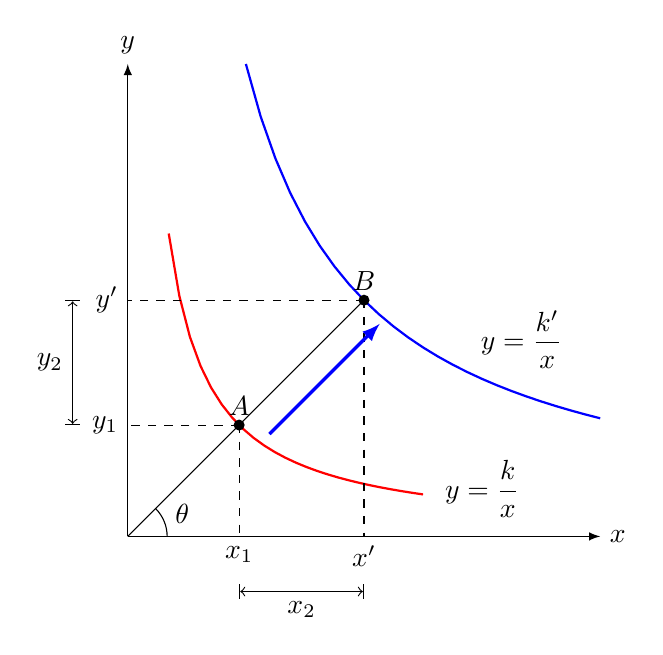
\begin{tikzpicture}
        \draw[-latex] (0,0) -- (6,0) node[right] {$x$};
        \draw[-latex] (0,0) -- (0,6) node[above] {$y$};
        \draw[domain=0.52:3.75, thick, red] plot (\x, {2/\x});
        \draw[domain=1.5:6, thick, blue] plot (\x, {9/\x});

        \coordinate (A) at ({sqrt(2)},{sqrt(2)});
        \coordinate (O) at (0,0);
        \coordinate (B) at ({sqrt(2)},0);
        \coordinate (C) at (0,{sqrt(2)});
        \coordinate (D) at (3,3);
        \coordinate (E) at (3,0);
        \coordinate (F) at (0,3);

        \fill (A) circle (2pt);
        \node[above] at (A) {$A$};
        \fill (D) circle (2pt);
        \node[above] at (D) {$B$};

        \draw (D) -- (O);
        \pic [draw, pic text=$\theta$, angle eccentricity=1.5] {angle = B--O--A};

        \draw[dashed] (A) -- (B);
        \draw[dashed] (A) -- (C);
        \node[below] at (B) {$x_1$};
        \node[left] at (C) {$y_1$};

        \draw[dashed] (D) -- (E);
        \draw[dashed] (D) -- (F);
        \node[below] at (E) {$x'$};
        \node[left] at (F) {$y'$};

        \node at (4.5,0.6) {$\displaystyle y=\frac{k}{x}$};
        \node at (5,2.5) {$\displaystyle y=\frac{k'}{x}$};
        
        \draw[-latex, very thick, blue] (1.8,1.3) -- (3.2,2.7);
        \draw[|<->|] ({sqrt(2)},-0.7) -- node[below] {$x_2$} (3,-0.7);
        \draw[|<->|] (-0.7,{sqrt(2)}) -- node[left] {$y_2$} (-0.7,3);

    \end{tikzpicture}
    \caption{添加流动性引起储备曲线缩放}
\end{figure}

反之,如果 LP 移除一部分流动性,那么变化方向就与上图相反。

添加或移除流动性使得流动性池的状态从 A 点移动到 B 点,使得储备曲线以原点为中心缩放,但没有改变价格。

在继续深入学习之前,我们先岔开话题,讨论一下为什么一定价格条件下对于确定规模的交易,流动性越大,滑点就会越小,交易引起的价格变化也越小。

视 $\Delta x$ 为外生变量,滑点用价差 $\displaystyle \left| \frac{\Delta x}{\Delta y} - \frac{x_0}{y_0} \right|$ 表示,价格变化用 $|p_X'-p_X|$ 表示,于是有

\begin{equation}
    \left| \frac{\Delta x}{\Delta y} - \frac{x_0}{y_0} \right|
     = \left| \frac{\Delta x}{y_0} \right|
\end{equation}
    
\noindent 当 $y_0$ 增大时,这个值显然会减小。

\begin{equation}
    |p_X'-p_X| = \left| \frac{x_0y_0}{(x_0+\Delta x)^2} - \frac{y_0}{x_0} \right| = \left| \frac{2x_0y_0\Delta x - y_0(\Delta x)^2}{x_0(x_0+\Delta x)^2} \right|
\end{equation}

\noindent 这个分式的分子是一个二次多项式,分母是一个三次多项式,当 $x_0,y_0$ 同比例增大时,分式的值显然会减小。

除了代数证明,也可以使用几何方法证明这两个规律,请读者自行尝试。

下面让我们回到正题,了解流动性代币与收益分配的机制。

一个流动性池可能有多个 LP ,我们往往需要按他们的贡献分配收益,这样才能保证公平公正。一位 LP 提供的流动性越多,最终获得的收益就越大。

为了把这个机制量化,我们引入了\textbf{流动性代币}(Liquidity Token)。流动性代币是一种特殊的代币,它衡量了 LP 对流动性池的贡献。用传统金融的术语来解释,它可以被视为所有者权益的凭证,或者简单理解成流动性池的股票。

当 LP 向流动性池添加流动性时,交易所会铸造一定数量的流动性代币发送给 LP 。当 LP 决定移除流动性时,他便可以将一定数量的流动性代币发送给交易所并赎回自己的份额,交易所将这一部分流动性代币销毁。

对于第一位 LP ,若其存入了 $x_0$ 个货币 X 和 $y_0$ 个货币 Y , Uniswap 使用公式

\begin{equation}
    s = \sqrt{x_0y_0}
\end{equation}

\noindent 计算其初始份额,也就是流动性代币数量。

对于第二位及以后的 LP ,若流动性池中已经有 $x_0$ 个货币 X 和 $y_0$ 个货币 Y ,已经铸造的流动性代币总量为 $s_0$ , 某位 LP 存入了 $x_1$ 个货币 X 和 $y_1$ 个货币 Y (无套利),Uniswap 使用公式

\begin{equation}
    \Delta s = \frac{x_1}{x_0} s_0 = \frac{y_1}{y_0} s_0
\end{equation}

\noindent 计算本次添加流动性铸造出的流动性代币数量,并使用 $s_0 \leftarrow s_0 + \Delta s$ 更新总的份额值。

提取流动性时,某位 LP 向流动性池发送数量为 $\Delta s$ 的流动性代币,自动做市商销毁这些代币,并将 $\Delta x$ 个货币 X 和 $\Delta y$ 个货币 Y 从流动性池中取出,发送给 LP ,其中 $\displaystyle \Delta x = \frac{\Delta s}{s_0} x_0, \Delta y = \frac{\Delta s}{s_0} y_0$ 。

这样的计算方式能够保证不存在无风险套利机会。无论价格怎样变化,各个 LP 的贡献总是得到了公平公正的评估,最终收益分配也是公平公正的。

\section{Uniswap 的相关风险}

\subsection{流动性不足}

现阶段, Uniswap 的流动性问题再怎么强调都不为过。前文已经提及,如果资金池的流动性不足,交易者会承受过大的滑点。这里我们再将相关危害拓展一下,探讨另外两个话题:三明治攻击和撤池跑路。

在传统金融市场中,抢先交易(Front Running)往往被认为是一种市场操纵行为。交易者向经纪商发送交易请求后,经纪商可以根据掌握的信息进行套利。下面是一个例子。

假设交易者委托经纪商以 1.1 美元购入 1 支股票,此时订单簿状况为

\begin{table}[htbp]
    \centering
    \begin{tabular}{lll}
        & 价格  & 数量 \\ \hline
        卖2 & 1.2 & 1  \\ \hline
        卖1 & 0.9 & 1 
    \end{tabular}
\end{table}

\noindent 经纪商得知交易者的订单后,用自己的资金以 0.9 美元买入 1 支股票,然后以 1.1 美元挂单卖出,再向交易所提交交易者的订单,使得交易者以 1.1 美元成交,从而赚取 0.2 美元的无风险利润。实际上,这 0.2 美元的福利应该归属于交易者,经纪商只是利用自己的信息霸权剥削了这一部分利润。

去中心化金融中也存在类似的攻击。在真实的 Defi 交易市场上,时间不是连续的,而是离散的,这是区块链的特性决定的。一笔交易往往是随着其他许多笔交易一起在同一个区块中处理。假如在一个区块中,两个交易者都针对同一个交易对发出了交易广播,那么这两笔交易的先后顺序就会影响各自交易的实际价格。如果交易者 A 先于交易者 B 完成购买,那么价格就会被推高,交易者 B 购买时获得的实际价格就会高于期望价格,承受更大的滑点。

区块链上没有经纪商,但是扮演类似角色的矿工可以在公共内存池中自由地选择若干笔交易并进行任意排序,而矿工自己也可以发送交易广播。如果矿工发现有利可图的交易序列,他就可以先用自有资金买入代币,然后将交易者的交易委托排在其后推高价格,并在区块的末尾将自己买入的代币以高价卖出,从而赚取无风险利润。这就是三明治攻击(Sandwich Attack)的原理,矿工的利润实质上直接侵害了交易者的利益。

\begin{figure}[htbp]
    \centering
    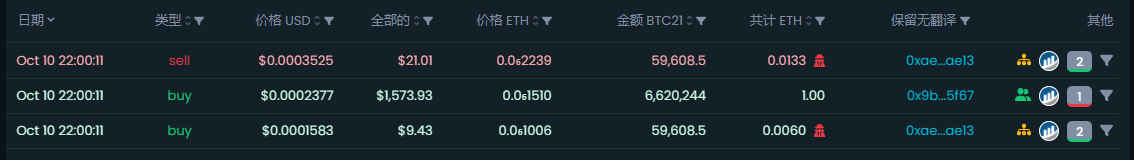
\includegraphics[width=14cm]{三明治攻击示意图.png}
    \caption{三明治攻击示意图}
\end{figure}

矿工并不能随心所欲地攻击获利,因为 Uniswap 会对每笔交易收取交易费,如果交易者的资金量很小,产生的价格推动效应并不能够弥补套利花费的两次手续费。因此,只要流动性足够大,交易者的价格推动效应就足够小,从而使得这种攻击无利可图。

下面介绍撤池跑路(Rug Pull)。

如果我们允许流动性提供者随时随地、随心所欲地移除流动性,那么这的确符合古典经济思想的美学和哲学——允许交易者自由地进入和退出市场。但是实际操作中,这种行为往往会被认为是不负责任的表现。

\begin{figure}[htbp]
    \centering
    \includegraphics*[width=10cm]{rugpull.jpeg}
    \caption{撤池跑路示意图}
\end{figure}

对于某些比较冷门的币种交易对,突然地撤出所有流动性将会使得交易者无法再参与交易,也就意味着代币的持有人无法将代币换为主流货币。当一个货币停止流通,其生命也就宣告终结。投资者持有的代币将变成一段无用的代码,化为一文不值的废品。Dextool 上记录的一天中产生的新池绝大多数的命运都是归零或撤池跑路。许多土狗项目或洗钱盘都会在募集一定资金后突然撤出所有流动性,让投资者措手不及。

一般来讲, LP 都是代币的长线投资者。为了证明自己长期持有代币的决心, LP 可以将铸造出的流动性代币发送到某个合约地址,并在合约中约定一定期限内不取出。这个操作称为锁仓(lock liquidity)。一个流动性池的锁仓率越高,其短期内发生大规模撤出流动性的可能性就越低。

需要指出的是, Uniswap 本身并不提供锁仓功能,它只是一个交易所而已。锁仓往往需要另外的合约框架来实现。

为了防范我们购买的代币或投资的项目发生意料外的撤池跑路,我们可以使用合约安全检测来保障我们的资金安全。一般来讲,诸如 Dextool 和 Ave.ai 的 Defi 信息平台都会提供自有的合约检测通道,在 Telegram 上也存在着许多自动检测机器人。但是我们不应该把鸡蛋放在同一个篮子里,毕竟,土狗项目方买通合约检测平台出具安全证明的现象广泛存在。即使所有合约检测工具都给出了安全证明,项目方依然有可能留下了某些 0day 漏洞可供利用。但无论如何,将各方面信息加以比较对照,总归是能提高安全性的。

\subsection{无常损失}

\textbf{无常损失}(Impermanent Loss)是由于交易对价格变化导致的相对于预期收益的机会损失。将 Impermanent Loss 巧妙地翻译为“无常损失”而不是“短暂损失”,其实传达了对 LP 们的风险警示。

假设 LP 投资的最终目标是获得尽可能多的美元。在 0 时刻, X/USD 价格为 $a_0$ , Y/USD 价格为 $b_0$ , LP 向流动性池中存入 $x_0$ 个货币 X 和 $y_0$ 个货币 Y ,并满足 $x_0y_0=k$ 。到 1 时刻,两个货币相对于美元的价格发生了变化, X/USD 价格为 $a_1$ , Y/USD 价格为 $b_1$ ,流动性池中有 $x_1$ 个货币 X 和 $y_1$ 个货币 Y ,并依然满足 $x_1y_1=k$ 。

\begin{equation}
    \begin{matrix}
        \left\{ 
            \begin{aligned}
                & X/USD = a_0 \\
                & Y/USD = b_0 \\
                & X/Y = \frac{x_0}{y_0}\\
                & x_0y_0 = k
            \end{aligned}
        \right.
        & \rightarrow &
        \left\{ 
            \begin{aligned}
                & X/USD = a_1 \\
                & Y/USD = b_1 \\
                & X/Y = \frac{x_1}{y_1}\\
                & x_1y_1 = k
            \end{aligned}
        \right.
    \end{matrix}
\end{equation}

忽略赚取的手续费,设 LP 在 0,1 时刻的资产(以 USD 计价)分别为 $B_0,B_1$ ,那么

\begin{equation}
    r = \frac{B_1}{B_0} 
    = \frac{a_1x_1+b_1y_1}{a_0x_0+b_0y_0} 
    = \frac{a_1^{\frac{3}{2}}b_1^{-\frac{1}{2}} + b_1^{\frac{3}{2}}a_1^{-\frac{1}{2}}}{a_0^{\frac{3}{2}}b_0^{-\frac{1}{2}} + b_0^{\frac{3}{2}}a_0^{-\frac{1}{2}}} 
    = \sqrt{\frac{a_0b_0}{a_1b_1}} \cdot \frac{a_1^2+b_1^2}{a_0^2+b_0^2}
\end{equation}

\noindent 即代表 LP 通过提供流动性带来的收益。很显然,若 $a_1>a_0,b_1>b_0$ ,则 $r>1$ , LP 必然获利;若 $a_1<a_0,b_1<b_0$ ,则 $r<1$ , LP 必然亏损;若 X 的价格和 Y 的价格呈负相关,则 LP 的损益情况还需进一步讨论,此处不做展开。

下面我们考虑 LP 不参与提供流动性,而只是简单持有代币,设其在 1 时刻的资产为 $B^* = a_1x_0+b_1y_0$ 。

\subsection{诈骗、假币与洗钱}

\subsection{价格预言机失灵}

\subsection{黑客攻击}

监守自盗

\end{document}

